
\documentclass[../D+Manual.tex]{subfiles}

%\externaldocument[P-]{Preface}
\begin{document}

\chapter{Getting started}
\label{sec:gettingstarted}

\begin{quote}
	The secret of getting ahead is getting started.\\
	\hspace*{\fill} \textit{Mark Twain (or not)}
\end{quote}

D+ computes the X-ray scattering from large supramolecular structures in solutions with high resolution.
Both geometric and atomic models can be computed and combined in hierarchical manner to form complex structures.
D+ can be launched either in remote mode or in local mode.
By default, D+ launches in local mode.
To launch D+ in the remote mode, run \path{DPlus.exe --remote}.
This can be simplified by creating a shortcut to \path{DPlus.exe} and adding \path{--remote} to the target or by creating a batch script doing the same.
If installed with the installer, there will be a \path{D+ Remote} shortcut in the Windows Start Menu.
Once everything is installed correctly, open D+. Two windows should open.
One looks like a command prompt, the other should look something like Figure \ref{fig:openingWindow}.

\begin{figure}[h!]
	\centering
	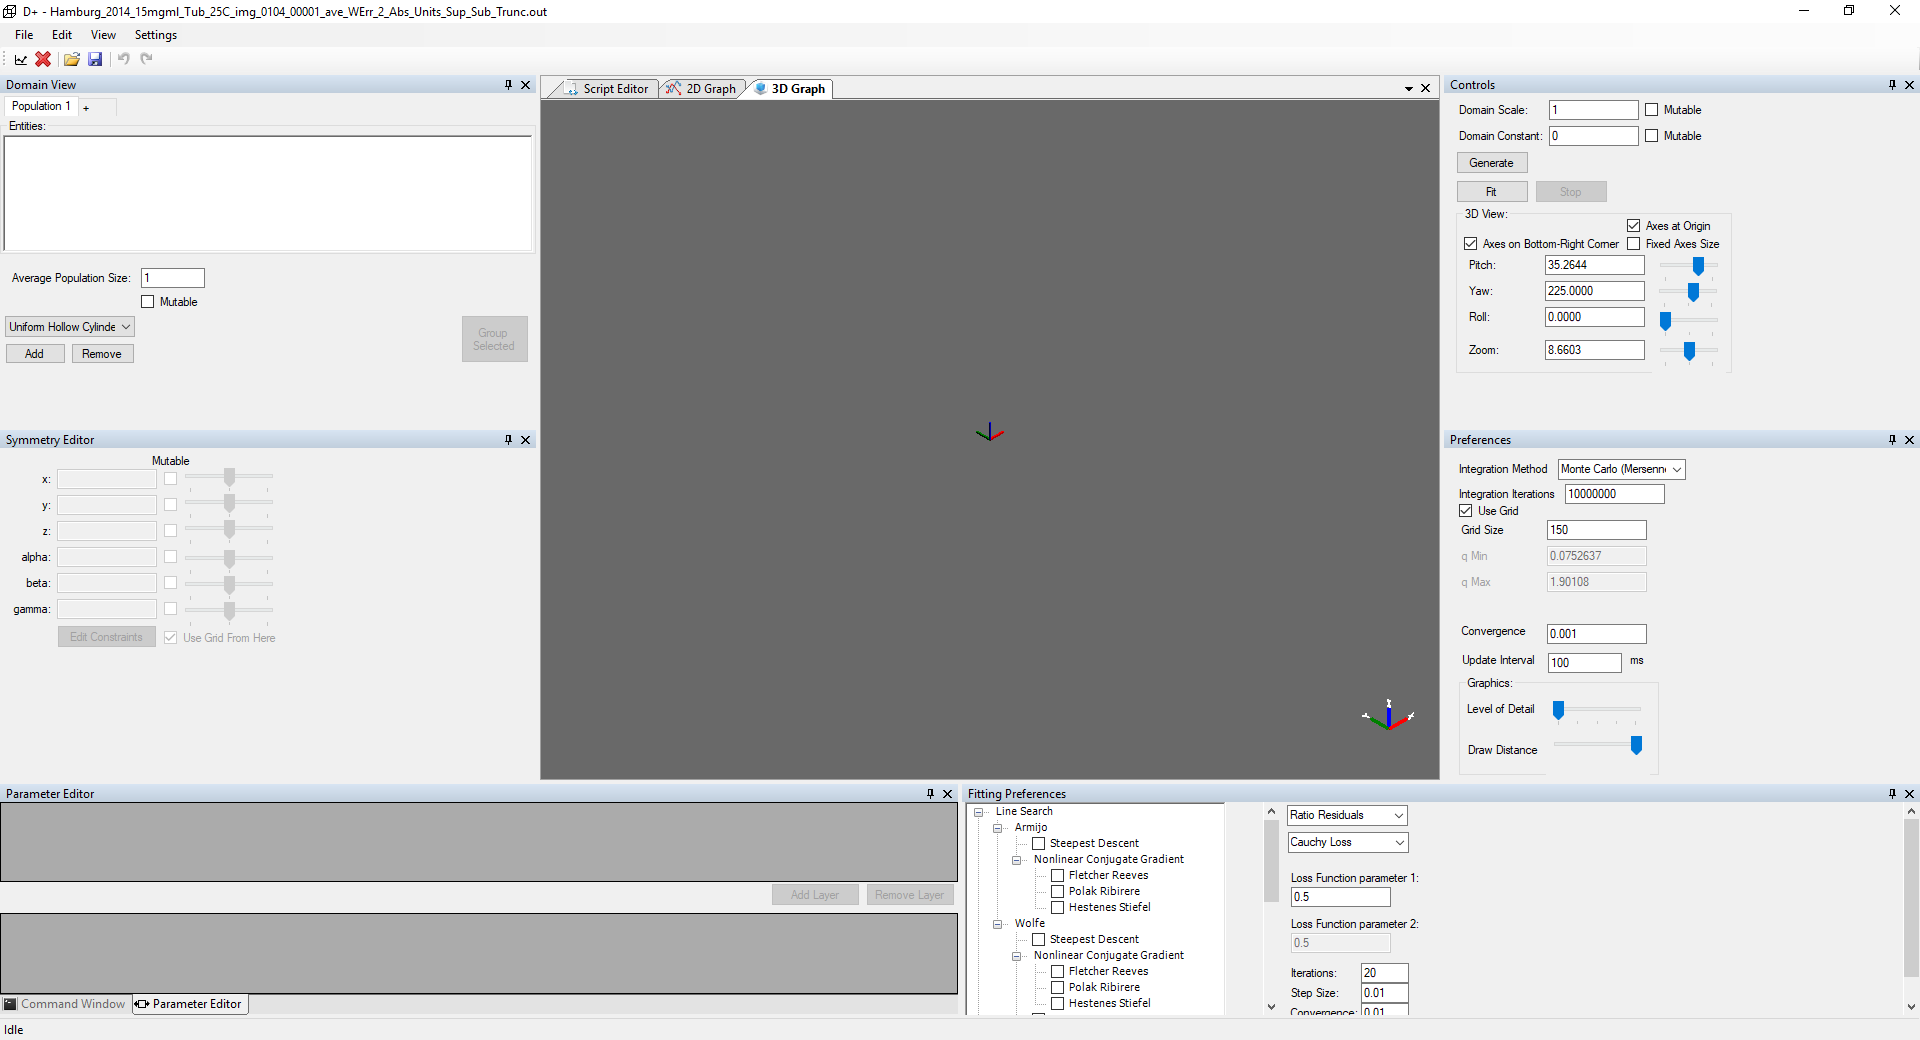
\includegraphics[width=0.635\textwidth]{openingWindow}
	\caption[The main window]{The main window contains multiple ``dockable'' tabs that can be placed based on personal preference. Each tab is addressed in this manual.}
	\label{fig:openingWindow}
\end{figure}

We shall address each of the panes here covering the various elements. The work-flow in D+ starts by defining a structure, continues by selecting the computation parameters, and ends by performing the computation itself. To help new users to get started, the folder of D+ has a \path{./Tutorials/} directory containing six tutorials, which cover the most important elements of D+. The \path{./Example Files/} directory includes several examples for the collective use of D+, some of which can be found in chapter \ref{chp:examples}. The \path{./LuaScripts/} directory has several examples of \href{http://www.lua.org/}{\texttt{Lua}} scripts, some of which can be found in chapter \ref{chp:scripts}. 

\section{Main window} \label{sec:mainWindow}


\begin{wrapfigure}{r}{0.3\textwidth}
	\vspace{-13pt}
	\centering
%	\fbox{
	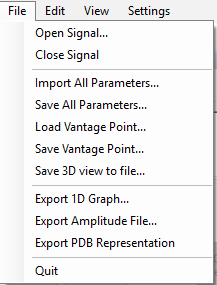
\includegraphics[width=0.95\linewidth]{fileMenu}
%	}
\end{wrapfigure}

There are a few functions that can be accessed from the main window.
Under the \path{File} menu, \path{Open Signal...} and \path{Close Signal} load and close an experimental signal against which the model will be plotted, compared with, and fit to.
\path{Save All Parameters...} saves all the parameters from the various panes (such as the \path{Domain View}, \path{Parameter Editor}, etc., but not from the \path{Script Editor}) to a file. The \path{Script Editor} has a separate save button. 
\path{Import All Parameters...} then loads all the parameters from that file and updates the graphic user interface (GUI).
\path{Save Vantage Point...} saves all the parameters from 3D view, (sec. \ref{sec:controls})
\path{Load Vantage Point...} then loads all the parameters from that file and updates the GUI.

The option \path{Save 3D view to file...} is not implemented.
\path{Export 1D Graph...} saves the calculated curve that is displayed in the \path{2D Graph} pane.
\path{Export Amplitude File...} and \path{Export PDB Representation} will be addressed in chapter \ref{sec:IntRes}.
\path{Quit} exits D+ (surprise!).


\begin{wrapfigure}[10]{r}{0.27\textwidth}
	\vspace{-15pt}
	\centering
%	\fbox{
	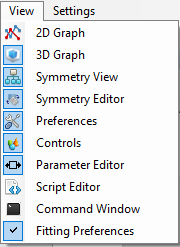
\includegraphics[width=0.95\linewidth]{viewMenu}
%	}
%  \caption{Basic layout}
\end{wrapfigure}
Figure \ref{fig:openingWindow} shows a possible layout of the main window.
Change the layout based on personal preference.
If a particular window or pane is closed, it can be reopened by going to the \path{View} menu and selecting the closed pane.
This also brings panes that are tabs behind other tabs to the forefront of the other tabs.
If you are looking for a pane that seems to have disappeared, this is a good place to help find it.

\begin{wrapfigure}{r}{0.25\textwidth}
	\vspace{-13pt}
	\centering
%	\fbox{
	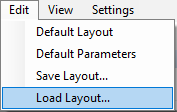
\includegraphics[width=0.95\linewidth]{editMenu}
%	}
\end{wrapfigure}
To save a particular layout, go to the \path{Edit} menu and select \path{Save Layout...}.
A layout can be loaded by selecting \path{Load Layout...}.
When closing D+, a file named \path{Latest.dlayout} will be created in the directory (or in \path) so that the layout is preserved from session to session.
The \path{Default Layout} is just a ``common ground'' layout and not a particularly comfortable one.
Create one that feels right for you and save your own layout. Similarly, there is also an option to restore the \texttt{Default Parameters} in \texttt{Controls}, \texttt{Preferences}, and \texttt{Fitting Preferences} panes.

\begin{wrapfigure}{r}{0.35\textwidth}
%	\vspace{-13pt}
	\centering
%	\fbox{
	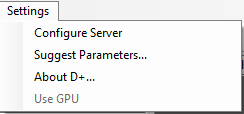
\includegraphics[width=0.95\linewidth]{settingsMenu}
%	}
\end{wrapfigure}
Other elements of the main window include the \path{Settings} menu and a status strip on the bottom of the  window.
%The \path{Settings} menu has two items that affect how the GUI is updated when fitting.
%The ``Live Generation'' option should never be checked.
%There is no good reason for its existence and should have been burninated long ago.
The \texttt{Configure Server} option allows you to specify the server address and activation code. \texttt{Suggest Parameters...} opens the Suggest Parameters tool that suggests computational parameters based on the dimensions of the computed object. \texttt{About D+...} provide information about the current version of D+. When the computer has a GPU card, \texttt{Use GPU} is active and enables the user to choose whether to use it or not.
The status strip at the bottom of the main opening window (Figure \ref{fig:openingWindow}) should just have the word \texttt{Idle} on the left, as there is nothing happening when opening D+.
Later when using D+, there may be different statuses as well as a progress bar.

\begin{wrapfigure}[2]{r}{0.25\textwidth}
	\vspace{-7pt}
	\centering
%	\fbox{
	
\includegraphics[width=0.95\linewidth]{mainWindowButtons}
%	}
\end{wrapfigure}

In addition to the menus, there is a row of buttons near the top of the main window. The left four (\path{Open Signal...}, \path{Close Signal}, \path{Open Parameter File...} and \path{Save Parameters}) correspond to menu items in the \path{File} menu. The \path{Undo} and \path{Redo} buttons are unimplemented.
% The right-most button (\path{Toggle console}) will open and close the window that looks like a command prompt. Note that closing it will result in its contents being cleared.
% This window is used to provide supplementary information when using D+ and can help in identifying problems when they arise.

\section{Domain View} \label{sec:domainView}

The \path{Domain View} window contains the list of models that will be used to calculate a solution Small Angle X-Ray Scattering (SAXS) curve. We shall go over each element here.

%\begin{wrapfigure}{r}{0.35\textwidth}
%	\vspace{-13pt}
%	\centering
%%	\fbox{
%    \begin{tabular}{@{}c@{}}
%    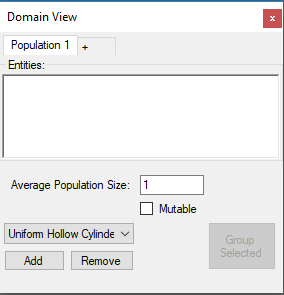
\includegraphics[width=0.95\linewidth]{DomainViewBlank} \\% Dummy image replacement
%    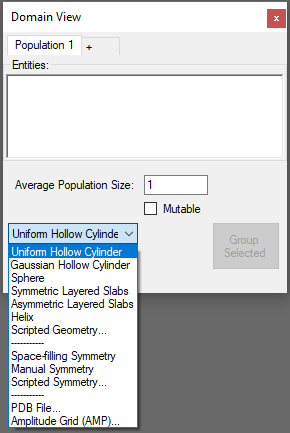
\includegraphics[width=0.95\linewidth]{DomainViewModelMenu} \\% Dummy image replacement
%  %  \textcolor{red}{\rule{3cm}{3cm}} \\% Dummy image replacement
%    \end{tabular}
%%	}
%\end{wrapfigure}

\begin{wrapfigure}{r}{0.35\textwidth}
	\vspace{-10pt}
	\hspace{-15pt}
	\centering
%	\fbox{
    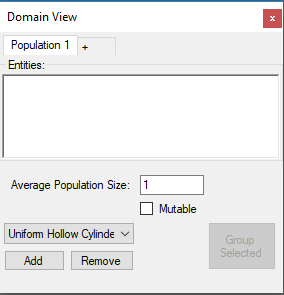
\includegraphics[width=0.95\linewidth]{DomainViewBlank}
%	}
\end{wrapfigure}

First, you will note that on the top, there is a tab called \texttt{Population 1}. Multiple populations can be used. Different populations are assumed to have no correlations between them and therefore the scattering intensities (rather than amplitudes) are summed. Within each population there are correlations between the positions and orientations of subunits and therefore the scattering amplitudes of subunits are added. For explanations regarding the difference, see the published literature \textcite{Ben-NunX+,als2011elements, Kittel2005}. Each population has an \texttt{Average Population Size} (default is 1). All the population sizes are given their respective weights, $w_i$, and the sum is divided by the total. In other words, the fraction of each population is given by $\nicefrac{w_i}{\sum w_i}$. To add a population, press the \texttt{+} button to the right of the tab(s). Populations can be renamed for convenience by right clicking on the population tab and choosing \path{Rename} or \path{F2} (the \path{F2} option requires using the mouse before being able to press \path{F2}). Populations can be deleted by center clicking on the relevant tab or choosing \path{Close Population} from the context menu. The Mutable checkbox refers to the \texttt{Average Population Size}.

\begin{wrapfigure}{r}{0.35\textwidth}
	\vspace{-20pt}
	\centering
%	\fbox{
    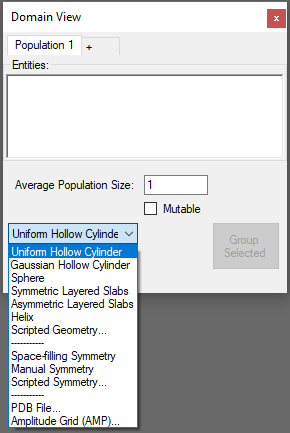
\includegraphics[width=0.9\linewidth]{DomainViewModelMenu}
%	}
\end{wrapfigure}

To add models to the population, select a model from the drop down menu on the lower left and press the \texttt{Add} button below it. Selected models can be renamed by right clicking on the model and choosing \path{Rename} or \path{F2}. The models are divided into three categories: geometric models; symmetries; and other. Other includes loading a \texttt{PDB file}, and loading a precalculated \texttt{Amplitude Grid (AMP)} from a file. To avoid incompatibility issues, when a precalculated amplitude is loaded, \texttt{q Max} and/or \texttt{Grid Size}, based on which the loaded amplitude was created, should not be further changed at the GUI. The grid is essentially a lookup table of amplitudes in the 3D reciprocal space ($\vec{q}$) used by D+ to calculate the scattering amplitude (and then intensity) of larger and more complex structures. Precise descriptions of the geometric models can be found in the paper ``Solution X-ray scattering form factors of supramolecular self-assembled structures'' \textcite{szekely2010solution}. The available geometric models are \texttt{Uniform Hollow Cylinder, Sphere, Symmetric Layered Slabs, Asymmetric Layered Slabs}, and \texttt{Helix}. After selecting a model and pressing \texttt{Add}, the model is included in the tree. Selecting the model provide access to \texttt{Parameter Editor}, in which the the electron density and dimensions can be provided. Additional layers of the same geometry can be added by pressing \texttt{Add Layer}. This bottom is in active in the \texttt{Helix} model. Layers can be added by using ``\textit{Symmetries}''.  The ``\textit{Symmetries}'' will be addressed in full in chapter \ref{chp:Symmetries}, but for now, just note that they must ``wrap'' other models. If one or more models are selected in the Entities box (from here on, the entity tree) and a \texttt{Symmetry} is selected in the drop down menu, the \texttt{Group Selected} button becomes active. Pressing it will ``wrap'' the selected model(s) in a new \texttt{Symmetry}. Models in the entity tree can be moved around by dragging and dropping. To remove a model, select it and press the \texttt{Remove} button or the delete key.

When the drop-down box is on \texttt{PDB File} or \texttt{Amplitude Grid (AMP)}, a \texttt{Center PDB} checkbox appears.
When loading a PDB with the box checked, the atomic coordinates are translated such that the center of mass coincides with the origin $\left(0,0,0\right)$. 
Centering the structure around the origin is important since it minimizes the number of grid points, $G$, and hence the \texttt{Grid Size}, which  are needed to satisfy the Nyquist-Shannon sampling rate (see more detail in section \ref{sec:preferences}).
Try it.
Download a PDB file from the \href{http://www.rcsb.org/pdb/home/home.do}{Protein Data Bank}.
Load the file with and without the checkbox checked. For an Amplitude File, the checkbox does not change anything except indicating that the box was checked in the headers of the resulting outputs.

\section{Symmetry Editor} \label{sec:symmetryEditor}

\begin{wrapfigure}{r}{0.35\textwidth}
	\vspace{-10pt}
	\centering
%	\fbox{
    \includegraphics[width=0.95\linewidth]{symmetryEditorBlank}
%	}
\end{wrapfigure}

When a single item (or model) is selected in the entity tree, the \texttt{Symmetry Editor} window is activated. The $x$, $y$, $z$ fields are the items location relative to the origin. The \texttt{alpha}, \texttt{beta}, and \texttt{gamma} fields dictate the orientation of the item, according to the convention of Tait -
Bryan. Starting from \texttt{gamma}, which dictates the rotation about the $z$ axis, followed by \texttt{beta}, which dictates the rotation about the $y$-axis and ending with \texttt{alpha}, which dictates the rotation about the $x$-axis. The rotation matrix is therefore:
\begin{gather*}
\mathbf{
A\left(\alpha,\beta,\gamma\right)=A_{x}\left(\alpha\right)\cdot A_{y}\left(\beta\right)\cdot A_{z}\left(\gamma\right)=}\\
\left[
\setlength\arraycolsep{2pt}
\begin{array}{ccc}
1 & 0 & 0\\
0 & \cos\left(\alpha\right) & -\sin\left(\alpha\right)\\
0 & \sin\left(\alpha\right) & \cos\left(\alpha\right)
\end{array}\right]%\\
\mkern-8mu\cdot\mkern-8mu
\left[
\setlength\arraycolsep{2pt}
\begin{array}{ccc}
\cos\left(\beta\right) & 0 & \sin\left(\beta\right)\\
0 & 1 & 0\\
-\sin\left(\beta\right) & 0 & \cos\left(\beta\right)
\end{array}\right]%\\
\mkern-8mu\cdot\mkern-8mu
\left[
\setlength\arraycolsep{2pt}
\begin{array}{ccc}
\cos\left(\gamma\right) & -\sin\left(\gamma\right) & 0\\
\sin\left(\gamma\right) & \cos\left(\gamma\right) & 0\\
0 & 0 & 1
\end{array}\right]=\\
\setlength\arraycolsep{3pt}
\begin{bmatrix}\cos \beta\cos \gamma & -\cos \beta\sin \gamma & \sin \beta\\
\cos \alpha\sin \gamma+\cos \gamma\sin \alpha\sin \beta & \cos \alpha\cos \gamma-\sin \alpha\sin \beta\sin \gamma & -\cos \beta\sin \alpha\\
\sin \alpha\sin \gamma-\cos \alpha\cos \gamma\sin \beta & \cos \gamma\sin \alpha+\cos \alpha\sin \beta\sin \gamma & \cos \alpha\cos \beta
\end{bmatrix}
\end{gather*}

The \texttt{Edit Constraints} button opens up a window allowing constraints to be set (only the absolute minimum/maximum are implemented). The \texttt{Use Grid From Here} checkbox is for ``Hybrid'' calculations and will be explained in more detail in section \ref{sec:hybrid}.

\section{Command Window} \label{sec:commandWindow}

The \texttt{Command Window} provides access to some of the inner workings of D+. It can also be used as a calculator. The language used is \href{http://www.lua.org/}{\texttt{Lua}}. For example, typing \lstinline[language={[5.0]Lua}]|math.pi^2| at the prompt gives \lstinline[language={[5.0]Lua}]|ans = 9.86960440108936|. Everything that can be written in a script can be entered here. See chapter \ref{chp:scripts} for details.

\section{Script Editor} \label{sec:scriptEditor}

This pane is a basic \href{http://www.lua.org/}{\texttt{Lua}} script editor. There are buttons to \texttt{Open}, \texttt{Save}, \texttt{Cut}, \texttt{Paste}, etc. The main advantage of this pane is the ability to run, pause and stop scripts. Breakpoints can also be set by using the \texttt{Add/Remove Breakpoint} button or by clicking next to the line numbers. See chapter \ref{chp:scripts} for details on scripting.



\section{Parameter Editor} \label{sec:parameterEditor}

\begin{figure}[h!] %{r}{0.5\textwidth}
%	\vspace{-10pt}
	\centering
%	\fbox{
    \includegraphics[width=0.55\linewidth]{parameterEditorBasicCylinder}
%	}
%	\vspace{-10pt}
	\caption{\texttt{Parameter Editor} pane. Upper panel contains the model parameters of each layer (e.g., size (\texttt{Radius} in this example) or electron density (\texttt{E.D.})). The lower pane contains extra global parameters that apply to all the layers. }
	\label{fig:ParameterEditor}
\end{figure}

The \texttt{Parameter Editor} is where the parameters of each node in the entity tree can be edited. When one entity is selected, its parameters appear here (Figure \ref{fig:ParameterEditor}). The upper panel contains a table of the model parameters. These parameters are often organized by layers, with the number of layers being variable. The bottom pane contains the \textit{Extra Parameters} which is a fixed number of parameters characteristic of each model.
\newpage
\section{3D Graph} \label{sec:3DGraph}

\begin{wrapfigure}{r}{0.6\textwidth}
	\vspace{-10pt}
	\centering
%	\fbox{
    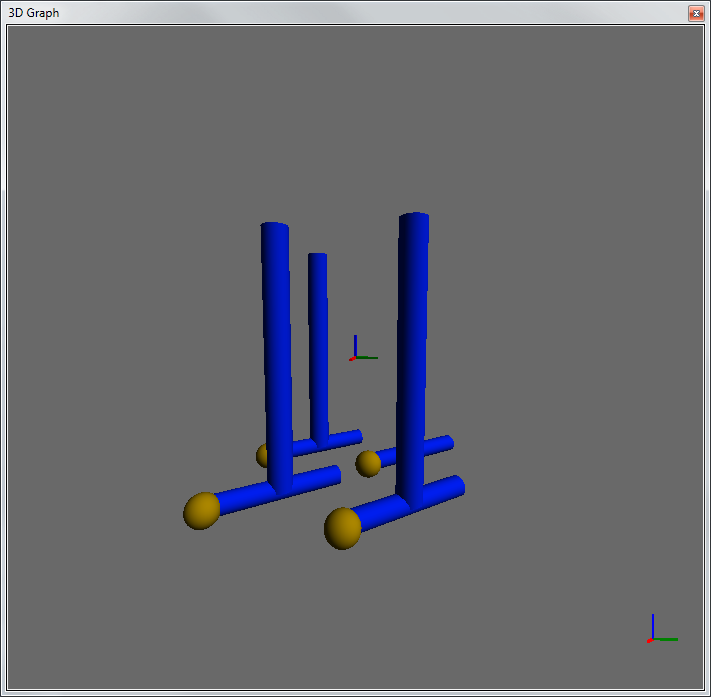
\includegraphics[width=0.6\linewidth]{3DGraph}
%	}
	\vspace{-10pt}
\end{wrapfigure}

The 3D Graph pane shows the real-space (or ``real-world'') picture whose solution X-ray scattering curve will be calculated. It can be rotated by holding down the right mouse button and dragging. Zoom is controlled by the scroll wheel. Items can be selected using the left mouse button. Dragging with the center mouse button changes the point upon which the camera focuses. Double clicking the center button returns the viewport to a semi-default setup. The camera can also be controlled from the \texttt{Controls} pane (sec. \ref{sec:controls}). Please note that if you have a large structure at atomic resolution it will take a long time to plot the 3D structure. It is better to work at minimal level of details and try to avoid the 3D Graph pane as much as possible.  

\section{2D Graph} \label{sec:2DGraph}

This window displays the calculated 2D graph of $I\left(q\right)$, which is the scattering  intensity, $I$, as a function of the magnitude of the scattering vector, $q$, of the model described in \texttt{Domain View}. The model is displayed in blue, while a loaded signal is red. A loaded signal is usually the signal that we are trying to fit. Note that you might want to check the \texttt{Log(i)} and/or \texttt{Log(q)} boxes for viewing the curves. You can zoom in by clicking on the left mouse button twice to define a rectangle you want to view. 


\section{Controls} 
\label{sec:controls}



The \texttt{Controls} pane contains two main parts. The lower part, labeled \texttt{3D View}, controls the camera for the 3D Graph (sec. \ref{sec:3DGraph}). There are the \texttt{Pitch}, \texttt{Yaw}, \texttt{Roll} and  parameters as well as \texttt{Zoom}. Three checkboxes, \texttt{Axes at Origin}, \texttt{Axes on Bottom-Right Corner}, and \texttt{Fixed Axes Size} control the display of the reference red, blue and green axes in the 3D Graph.

\begin{wrapfigure}{r}{0.35\textwidth}
	\vspace{-10pt}
	\centering
%	\fbox{
    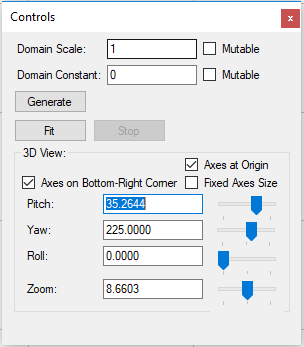
\includegraphics[width=0.95\linewidth]{controls}
%	}
	\vspace{-10pt}
\end{wrapfigure}
%TODO update 'Controls' figure (because the Single Geometry Mode has been removed).
The second (upper) part controls the generation and fitting of models. The domain scale (and its mutability checkbox) is a scale that the entire model is multiplied by. The Domain constant (and its mutability checkbox) is a constant that is added to the entire model. The \texttt{Generate} button starts the calculation of the current model. \texttt{Fit} will attempt to change the mutable parameters such that the model will better fit the loaded signal. The \texttt{Stop} button signals the calculation to abort. Note that stopping may not be immediate, (in particular when using GPU). 
\newpage
\section{Preferences} \label{sec:preferences}

\begin{wrapfigure}{r}{0.35\textwidth}
	\vspace{-10pt}
	\centering
%	\fbox{
    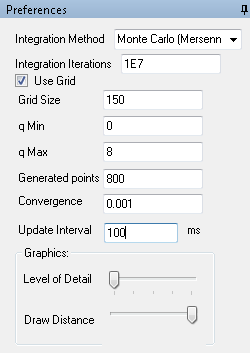
\includegraphics[width=0.95\linewidth]{preferences}
%	}
	\vspace{-10pt}
\end{wrapfigure}

The \texttt{Preferences} pane controls several parameters regarding the calculation of the modeled solution X-ray scattering curve. The \texttt{Integration Method}, \texttt{Integration Iterations}, and \texttt{Convergence} fields control how D+ calculates the orientation average of the model (more on this in chapter \ref{chp:integrationMethods}). The \texttt{Use Grid} checkbox determines whether or not lookup tables are allowed to be used in the calculations. Unchecking it may cause certain selection combinations not to work (\texttt{Adaptive (VEGAS) Monte Carlo}, for example). 

\texttt{q Max} and \texttt{q Min} are the greatest and lowest $q$ values for which the scattering intensity curve of the model will be calculated.
Only when no signal is loaded, \texttt{q Max} and \texttt{q Min} can be modified. If a signal is loaded the \texttt{2D Graph} pane will show a curve. If there is a loaded signal and \texttt{q Max} and/or \texttt{q Min} should be change, the signal should be removed by the \texttt{Close Signal} option in the \texttt{File} menu or by pressing the thick red \texttt{X} button near the top of the main window.  
The default value of \texttt{q Min} is $0$. In the current version, changing \texttt{q Min} does not affect the grid, which still contains all the points from 0 to \texttt{q Max}, hence the \texttt{Grid Size} parameter (which can be calculated by the  \texttt{Suggests Parameters} tool, explained in sec. \ref{SugPar}), should be computed assuming $q_{\text{min}} = 0$. Orientation average is computed only between $q_{\text{min}}$ and $q_{\text{max}}$. \texttt{Generated Points (resSteps)} determines the number of points on the $q$-axis that will be generated (note that in the \texttt{state file}, which saves the GUI parameters, this variable is called \texttt{resSteps}). 800 generated points is the default and D+ reverts back to 800 when reopened (even when loading a saved state). Note that \texttt{q Min}, \texttt{q Max}, and \texttt{Generated Points (resSteps)} parameters will be hidden when a signal is loaded as they will be determined based on the $q$-axis of the loaded signal. 

At the bottom of the pane there are two controls that affect the 3D Graph pane, \path{Draw Distance} and \path{Level of Detail}. If the \path{Level of Detail} is too high, rendering the scene (i.e, generating the image of the real-space model) will take a long time. 

\section{Fitting Preferences} \label{sec:fittingPreferences}

\begin{wrapfigure}{r}{0.5\textwidth}
	\vspace{-20pt}
	\centering
%	\fbox{
    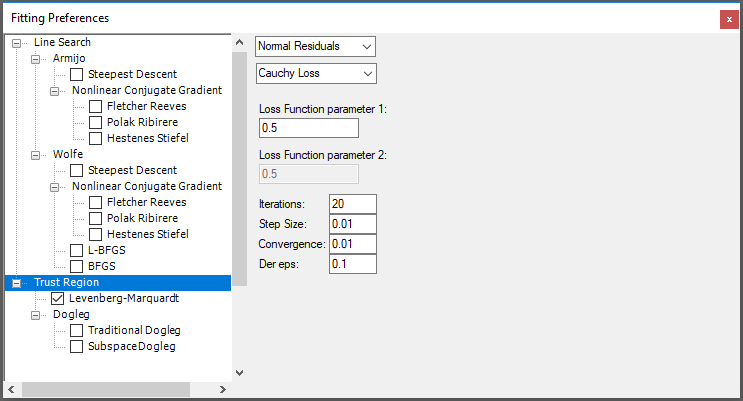
\includegraphics[width=1.1\linewidth]{fittingPreferences}
%	}
	\vspace{-10pt}
\end{wrapfigure}

D+ uses \href{http://ceres-solver.org/nnls_tutorial.html#}{\texttt{Ceres-Solver}} to try to fit mutable parameters to the data signal. This pane allows access to the various methods \href{http://ceres-solver.org/}{Ceres-Solver} uses to solve the non-linear least-squares problem:

\begin{equation*}
\begin{split}\min_{\mathbf{X}} &\quad \frac{1}{2}\sum_{i} \rho_i\left(\left\|f_i\left(x_{i_1}, ... ,x_{i_k}\right)\right\|^2\right) \\
\text{Subject to:} &\quad l_j \le x_j \le u_j\end{split}
\end{equation*}

\noindent where $x_i$ are the mutable variables.
In our case, the sum over $i$ is just a single term or Residual Block in \href{http://ceres-solver.org/}{Ceres-Solver} terminology.
$f_i(\cdot)$ is a Cost-Function that produces the residuals of the objective function (and calculates the Jacobian when asked).

The initial input includes the experimental scattering intensity  $I_\text{experimental}\left(q_i\right)$, an object that computes the expected scattering intensity  $I_\text{model}\left(q_i\right)$, and a functor that evaluates the residuals.
The residuals, $f_i$, can either be the \texttt{Normal Residuals}, $I_\text{experimental} - I_\text{model}$,
a \texttt{Ratio Residuals}
\begin{equation*}
1-\left(\frac{I_\text{experimental}}{I_\text{model}}\right)^{\pm 1},
\end{equation*}
where the $\pm$ is chosen so that the residual is non-negative, or a \texttt{Logarithmic Residual},
\begin{equation*}
\left|\log\left(\frac{I_\text{experimental}}{I_\text{model}}\right)\right|.
\end{equation*}
 
$\rho_i\left(\cdot\right)$ is a Loss-Function that can be chosen by the user.
The complete standard set of Loss-Functions (\texttt{Trivial Loss}, $\rho(s)=s$; \texttt{Huber Loss}, $\rho(s)=s$ if $s \le 1$ and $\rho(s)=2\sqrt{s}-1$ if $s>1$; \texttt{Soft L1 Loss}, $\rho(s)=2\left(\sqrt{1+s}-1\right)$;  \texttt{Cauchy Loss}, $\rho(s)=\log \left(s+1\right)$, etc.) from \href{http://ceres-solver.org/}{Ceres-Solver}, is available in the GUI of D+. Cauchy, for example, provides a robust curve fitting as it can deal with outliers in the data (see \href{http://ceres-solver.org/nnls_modeling.html}{\texttt{Ceres-Solver}}).
The method with which \href{http://ceres-solver.org/nnls_solving.html}{Ceres-Solver} tries to fit to the data can also be chosen from several methods including \texttt{BFGS}, \texttt{LBFGS}, \texttt{Levenberg-Marquardt}, or \texttt{Dogleg}. 
Upper and lower bound constraints for each mutable fitting parameter are also supported by  \href{http://ceres-solver.org/nnls_solving.html}{Ceres-Solver}. Place the mouse cursor on a mutable parameter and right click on the mouse to obtain a new window in which the bounds can be added. 

The (black) \texttt {Command Prompt} window will display messages when problems occur. The combination of \texttt{Lose}- and \texttt{Cost-Function} parameters dictate how the fitting will be performed when pressing the Fit button in the \hyperref[sec:controls]{\texttt{Controls}} pane.

The variables that control the fitting algorithms are \texttt{Step Size} that sets a limit on the fraction by which mutable parameters can be changed, \texttt{Iterations} - the maximum number of fitting attempts, \texttt{Convergence} - the cost function cutoff standard, and \texttt{Der eps}, which regulates the value of \texttt{Step Size} based on the change in the value of the cost function. The values of these variable should be adjusted and optimized for each case. Examples are provided in the paper of D+ and its supporting information. 

D+ can find the \textit{local} minimum for a plausible set of initial guess model parameters. Finding the initial guess should be done by several \texttt{Generate} iterations.
Alternatively, one can use the \hyperref[python-fitting]{\texttt{python API}} of D+ to generate the scattering curves and do the optimization or fitting using the available fitting algorithms of  Python, which may also include \textit{global} fitting algorithms. 

Fitting with certain options (for example, the thickness of a solvation layer) can take a significant amount of time (hours). When this is the case, it is better to use educated guesses. For small solvated structures (like soluble proteins), fitting with CRYSOL of FoXS is faster than D+ as no grids are computed in those programs.

To better know how to use the various combination of options and parameters see, for example,  \href{http://ceres-solver.org/}{Ceres-Solver}.


\section{Suggest Parameters}
\label{SugPar}
D+ has a \texttt{Suggest Parameters} tool under the \texttt{Settings} menu, located at the main window.
The tool gets as an input, \texttt{q Max}, and the \texttt{x}, \texttt{y}, and \texttt{z} coordinates of the point, $P$, which is most distant from the origin in the structure, for which grids are going to be used. 
If grids are used for the entire structure, $P$  should be the most distant point in the entire structure. However, when the Hybrid method is used, $P$ should be the most distant point in the part of the structure for which grids are used.  

The tool computes the distance, $L$, of the most distant point from the origin. 
\noindent Practically, $L$ is the higher of the following two value: the longest dimension in the structure (if the structure is centered around the origin - twice the radius of the sphere including the structure), or the most distant point from the origin in the structure. 
The \texttt{Suggest Parameters} tool can then compute, using Eq. \ref{eq:NumberofGridShells}, the suggested \texttt{Grid Size} for computations that use grid. 

The number of points in the 3D grid, $G$ (note the $G$ is not \texttt{Grid Size}), is a measure of how dense the reciprocal-space grid (or lookup table) will be. 
$G$ should be calculated according to the length of the structure $L$, contributing the highest frequency oscillation to the amplitude:
\begin{equation*}
G\approx \left[\left(2q_{\text{max}}\right)^3-\left(2q_{\text{min}}\right)^3\right]\cdot \left(\frac{L}{2\pi}\right)^3.
\label{eqn:GridDensity}
\end{equation*}

$q_\text{max}$ and $q_\text{min}$ are the maximum and the minimum magnitudes of the scattering vector, respectively. In the current version of D+ the number of grid points is calculated assuming  $q_\text{min}=0$, even when this is not the case. 
Note that this Nyquist-Shanon sampling rate is a rule of thumb, sometimes a denser grid is required. Further note that it is faster to compute structures (simple or complex) when their center of mass is at the origin, as smaller grid size will be required. 

Using \texttt{q Max}, 
and the \texttt{x}, \texttt{y}, and \texttt{z} coordinates of the most distant point in the structure (with respect to the origin), or the longest dimensions of the structure in \texttt{x}, \texttt{y}, \texttt{z} (the larger of the two options),  \texttt{Suggest Parameters} tool returns the \texttt{Grid Size} parameter, needed for D+, by computing:
\begin{equation}
\texttt{Grid Size} = 2N =  \left(\left[\frac{\left(q_{\text{max}}-q_{\text{min}}\right)\cdot L +3}{10}\right]+1\right)\cdot 10.
\label{eq:NumberofGridShells}
\end{equation}
where $N$ is the number of spherical grid shells. Therefore, there will be $N$ points between the origin (or $q=0$) and \texttt{q Max}, not including the origin. The reciprocal space grids have both negative and positive values of $\vec{q}$. The \texttt{Grid Size} parameter in D+ should therefore be an even number. If the \texttt{Grid Size} is an odd number, an error message is sent, in which the user is asked to modify the \texttt{Grid Size} to an even number.
Equation \ref{eq:NumberofGridShells} returns an integer number, which is divisible by 10.

\begin{wrapfigure}{r}{0.7\textwidth}
	\vspace{-10pt}
	\centering
	%	\fbox{
	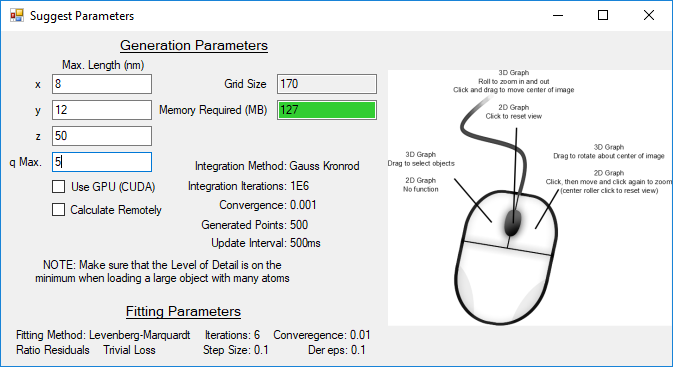
\includegraphics[width=0.95\linewidth]{SuggestParameters}
	%	}
	\vspace{-10pt}
\end{wrapfigure}

The \texttt{Suggest Parameters} tool also returns the RAM volume (in units of MB) that is required for storing the \texttt{Grid}. 

It also suggests the suitable orientation average \texttt{Integration Method}, based on the aspect ratio of the structure and if GPU or CPU are used. Adaptive integration methods (\texttt{Gauss Kronrod} for CPU or \texttt{Vegas Monte Carlo} for GPU) are more suitable when the structure has a high aspect ratio.

The tool also suggests the number of \texttt{Integration Iterations} that should be used in D+, the \texttt{Convergence} cutoff, the number of \texttt{Generated Points} within the required $q$ range, and the \texttt{Update Interval}, which the time in units of \texttt{ms} between successive computation updates. 

If the diameter of the sphere that envelopes the structure is larger than $L$, the \texttt{x}, \texttt{y}, and \texttt{z} coordinates should be such that the resulting $L$ will be that diameter. In that case, the integration parameters may not be optimal.

When the structure in not centered around the origin these suggestions are inaccurate, more details can be found in chapter \ref{chp:integrationMethods}).
In any event, the suggested parameters are only a guide or first approximation. In practice, higher or lower values might be more appropriate for optimal results. 

At the bottom of the \texttt{Suggest Parameters} pane, fitting method and \text{Fitting Parameters} are also suggested. These include the maximum number of \texttt{Iterations}, the fitting \texttt{Convergence} cutoff, the \textit{cost} and \textit{loss} functions, their maximum \texttt{Step Size} between fitting iterations, and its regularization parameter \texttt{Der eps}. 

On the right side of the pane, there are detailed explanations of how to use the mouse in D+ to control the presentation in both \texttt{2D} and \texttt{3D Graph} views.   

\section{PDBUnits}
\label{PDBUnit}

\texttt{PDBUnits} is an accessory tool that can be used to identify the orientation and translations
(or \hyperref[chp:Symmetries]{\texttt{Assembly Symmetry}}) of a repeating subunit (given in \texttt{Subunit PDB file} in a complex supramolecular structure (given in a \texttt{Large PDB file}). The program also gets the tolerance, given by the maximum root-mean-squared-displacement (\texttt{RMSD})
value, within which repeating subunits can be considered similar. 
The program reads the PDB file of the complete structure and finds all the instances
of the subunit. If subunits are splitted at different location in a PDB file, the parts
should be combined into complete subunits, before using the tool. 
For each instance the
rotation and translation with respect to the original subunit are computed. The tool
exports the \hyperref[chp:Symmetries]{\texttt{Assembly Symmetry}} of the subunit as a docking list (DOL) text
file, which is a required input for D+, to compute the entire structure using
the RG algorithm\cite{RGs2016}. 

The \texttt{*.dol} text file contains a list of the center of mass coordinates, \texttt{x}, \texttt{y}, and \texttt{z}, and the Tait–Bryan rotation angles \texttt{$\alpha$}, \texttt{$\beta$}, and \texttt{$\gamma$} about the corresponding axes, of each subunit instance, within the large PDB file. 

The program asks for the following items:
\begin{itemize}
	\item The complete structure as a \texttt{Large unit PDB file} path
	\item The \texttt{Subunit PDB file} path
	\item The \texttt{RMSD} value, which sets the maximum \texttt{RMSD} allowed difference between the given \texttt{Subunit PDB file} and any instance of the subunit, within the \texttt{Large unit PDB file}.
	\item The \texttt{Output DOL file path}, in which the list of translations and rotations of repeating subunit instances will be stored.   
\end{itemize}

The program can also be used from the \texttt{Command Prompt}. The default file path is: 

\texttt{C:$\backslash$Program Files$\backslash$D+$\backslash$bin>}

Within the folding, typing 
\texttt{PDBUnits --help}

gives the command line format: 
	
\texttt{PDBUnits <Large unit PDB file> <subunit PDB file> <RMSD> <Output DOL file path>}

\section{The Dplus Python API}\label{the-dplus-python-api}

The D+ Python API allows using the D+ backend from Python, instead of
the ordinary D+ application.

The Python API works on both Windows and Linux.

\subsection{Installation}\label{installation}

Installing the Python API is done using PIP:

\begin{lstlisting}[language=bash,basicstyle=\small, breaklines= true, breakatwhitespace= true]
pip install dplus-api
\end{lstlisting}

The API was tested with Python 3.5 and newer. More details are provided in a separate \href{https://scholars.huji.ac.il/uriraviv/book/python-api}{README file}.

\end{document}


